\documentclass[a4paper,12pt]{article} 



\usepackage[utf8]{inputenc}
\usepackage[english, russian]{babel}
\usepackage{caption}
\usepackage{listings}
\usepackage{amsmath,amsfonts,amssymb,amsthm,mathtools }
\usepackage{wasysym}
\usepackage{graphicx}
\usepackage{float} 
\usepackage{wrapfig} 
\usepackage{fancyhdr} 
\usepackage{lscape}
\usepackage{xcolor}
\usepackage[normalem]{ ulem }
\usepackage{hyperref}





\hypersetup
{
    colorlinks = true,
    linkcolor = blue,
    filecolor = magenta,
    urlcolor = blue
}


\pagestyle{fancy}
\fancyhead{}
\fancyhead[L]{ 2.2.8 }
\fancyhead[R]{ Талашкевич Даниил, 2 положительная группа крови}
\fancyfoot[C]{ \thepage }



\begin{document}


\begin{titlepage}

\newpage
\begin{center}
\normalsize Московский физико - технический институт //госудраственный университет)
\end{center}

\vspace{6em}

\begin{center}
\Large Домашняя работа по Физической культуре\\
\end{center}

\vspace{1em}

\begin{center}
\large \textbf{ Исследование термических эффектов,
возникающих при упругих деформациях[2.2.8] }
\end{center}

\vspace{2em}

\begin{center}
\large П$ ^ 3$ : Полная Полтрашка Патриковна и Талашкевич Даниил Александрович \\
Группа Б01 - \href{ https://vk.com/rt_kiska }{\textbf{Гладим киску каждый день}}
\end{center}

\vspace{\fill}

\begin{center}
    \large Иерусалим \\ 2 век до н.э.
\end{center}

\end{titlepage}



    \thispagestyle{empty}
    \newpage
    \tableofcontents
    \newpage
    \setcounter{page}{1}


\section{Введение в историю Иерусалима}

Древнейшая часть Иерусалима была заселена в 4 - м тысячелетии до н.э., что делает его одним из древнейших городов мира.За свою долгую историю, Иерусалим был как минимум дважды разрушен, 23 раза осаждён, 52 раза атакован и 44 раза завоёван либо вновь отвоёван.В разное время городом владели Израильское царство, Иудейское царство, Вавилон, Персидская империя и империя Александра Македонского, Египет Птолемеев, Сирия Селевкидов.После еврейского восстания во II веке до н.э.на некоторое время было восстановлено Иудейское Царство, но уже в 6 году н.э.на месте него была провозглашена римская провинция Иудея. Вслед за распадом Римской империи, Иерусалим отошёл к Византии.После Византии город принадлежал арабским халифатам, крестоносцам, государствам Айюбидов и мамлюков, Османской и затем Британской империям, Иордании и, наконец, Израилю. Учитывая центральное место, отводимое Иерусалиму как еврейским(сионизм), так и палестинским национализмом, на избирательность, неизбежную при резюмировании более чем 5000 - летней истории его населённости, часто накладывается идеологическая предвзятость или предшествующий опыт авторов.Еврейские периоды истории города важны для израильских националистов, дискурс которых предполагает, что современные евреи происходят от израэлитов и Маккавеев в то время как исламский, христианский и другие нееврейские периоды его истории важны для палестинского национализма, дискурс которого производит современных палестинцев от всех разнообразных народов, населявших регион В результате каждая из сторон утверждает, что история города была политизирована оппонентами, дабы подкрепить притязания последних на город, и что это подтверждается разностью акцентов, придаваемых различными авторами разнообразным событиям и эрам в истории города.

\section{Как древние греки считали производные}
Для того, чтобы вычислять производную греки поступили очень умно : они построили машину времени, переместились в 2021 год н.э., затем на крысичях украли мой 	extbf{ exe } - шник и данную статью с подробнейшим описанием как искать ее в 2021 году, затем вернулись обратно и сковозь долгие годы они научились все - таки ее брать.Вы наверное подумаете, что это все чисто воды обман и выдумка, но у меня есть на то доказательства : \newpage

 \begin{figure}[h]
 \center{ 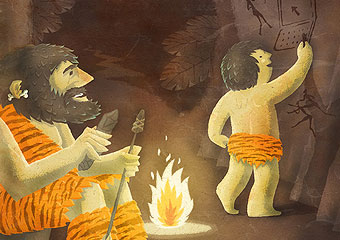
\includegraphics[scale = 1]{proof.jpg} }
 \label{ photo1:1 }
 \end{figure}

 На данном фото видно, как они внаглую просто переписывают мой код!!!! P.S.Фото взято из архивов национального музея наследний ЮНЕСКО

\section{Заключение}
 При выполнение домашней работы по физической культуре я узнал про историю Иерусалима, познакомился с тем, как греки считали производные, а так же сам научился считать производную по шагам!
\section{Используемые тренажеры}
 \begin{enumerate}
 \item Скакалка
 \item Эскандер
 \item Крижометр (отдельное спасибо Крижовичу за то, что предоставил его мне!)
 \item Коксовая дорожка
 \end{enumerate}
\end{document}
